\section{Module 2: Lecture 8\\Convolution Property of the Fourier Transform}

\subsection{Introduction}
In this lecture, we will talk about the properties of the Fourier transform and specifically, we see more about the convolution property.
\subsection{Convolution Theorem}
If two signals $x_1(t)$ and $x_2(t)$ both have Fourier transforms, which are $X_1(\Omega)$ and $X_2(\Omega)$ respectively, and if their convolution also has a Fourier transform, then this Fourier Transform is equal to the product $X_1(\Omega). X_2(\Omega)$.\\
Mathematically,
\begin{eqnarray}
x_1(t)\xrightarrow{F}& X_1(\Omega)\\
x_2(t)\xrightarrow{F}& X_2(\Omega)\\
x_1(t)*x_2(t)\xrightarrow{F}& X_1(\Omega).X_2(\Omega)
\end{eqnarray}
So, when we apply it to the context of the Linear Shift Invariance (LSI) system, we get
\begin{figure}[ht]
\centering
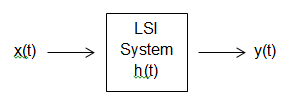
\includegraphics{fig0.png}
%\caption{\label VVoltage generator (side view)}
\end{figure}
\\
\begin{equation}
Y(\Omega)=X(\Omega)H(\Omega)
\end{equation}
where,
\begin{eqnarray}
x(t) &\xrightarrow{F}& X(\Omega)\\
y(t) &\xrightarrow{F}& Y(\Omega)\\
h(t) &\xrightarrow{F}& H(\Omega)
\end{eqnarray}
We said that there is a point-wise decoupling or memory less-ness in the Fourier domain, meaning, the output at angular frequency $\Omega$ depends only on the input at angular frequency $\Omega$ and the impulse response at angular frequency $\Omega$ and none other.\\
Where does this come from?\\
\indent $X(\Omega)$ is the component of input at angular frequency $\Omega$. Let us imagine $X(\Omega).ej\Omega t$ as input to the LSI system, where $X(\Omega)$ is a complex number.\\
Notionally,
\begin{figure}[h!]
\centering
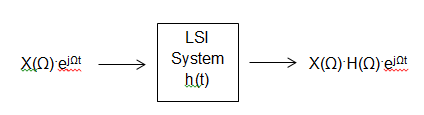
\includegraphics{fig1.png}
%\caption{\label VVoltage generator (side view)}
\end{figure}
\\
\begin{eqnarray}
y(t) &=& \int_{-\infty}^{\infty}h(\tau).X(\Omega).\textrm{exp}(j\Omega (t-\tau))d\tau\\
y(t) &=& \left( \int_{-\infty}^{\infty}h(\tau).\textrm{exp}(-j\Omega \tau)d\tau\right) X(\Omega).\textrm{exp}(j\Omega t)\\
y(t) &=& X(\Omega).H(\Omega).\textrm{exp}(j\Omega t)
\end{eqnarray}
$H(\Omega)$ is the component of the impulse response along $ej\Omega t$. Hence, $X(\Omega).H(\Omega)$ is the component $ej\Omega t$ in $y(t)$ and is equal to $Y(\Omega)$.\\
\begin{equation}
Y(\Omega)=X(\Omega).H(\Omega)
\end{equation}
This is analogous to an operator acting upon a force in mechanics. If $\nabla$ is the operator and if $\vec{F}$ the force vector such that
\begin{equation}
\vec{F}=F_x \hat{x} + F_y \hat{y} + F_z \hat{z}
\end{equation}
Then
\begin{eqnarray}
\nabla . \vec{F} &=& \nabla . (F_x \hat{x} + F_y \hat{y} + F_z \hat{z})\\
\nabla . \vec{F} &=& \partial_x F_x \hat{x} + \partial_y F_y \hat{y} + \partial_z F_z \hat{z}\\
\end{eqnarray}
Similarly we resolve the input into its components along the different $\Omega$'s, i.e. $ej\Omega  t$.
\begin{eqnarray}
x(t)&=&\sum_i X(\Omega_i).\textrm{exp}(j\Omega_i t)\\
y(t)&=&\sum _i X(\Omega_i).H(\Omega_i).\textrm{exp}(j\Omega_i t)
\end{eqnarray}
In a way, the idea is to decouple the action of the LSI system when we think of the input as comprising of different complex exponentials rotating at different angular frequencies, both positive and negative.
\subsection{What is a transform?}
More generally, transform is a change of paradigm. Paradigm means world view. In a system point of view, a signal is a mapping from the independent variable to complex numbers, while a system is a mapping from signals to signals. Whereas a transform is a mapping of the signals and systems altogether to the transformed domain of signals and systems.
\subsection{Convolution or Multiplication}
Doing multiplication, in general, is easier than convolution. To find find the convolution, take Fourier transforms of the two signals, multiply them and then take its inverse Fourier transform.
\begin{eqnarray}
x_1(t) &\xrightarrow{F}& X_1(\Omega)\\
x_2(t) &\xrightarrow{F}& X_2(\Omega)\\
X_1(\Omega).X_2(\Omega) &\xrightarrow{F^{-1}}& x_1(t).x_2(t)
\end{eqnarray}
It is beneficial only if the Fourier transform operations are easier to perform, otherwise it is not always better to go through the Fourier domain.\\
For example, take $x1(t)=x2(t)$ as a rectangular pulse as shown in the figure below.
\begin{figure}[h!]
\centering
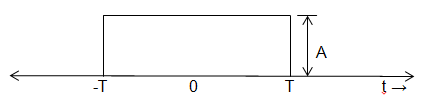
\includegraphics{fig2.png}
%\caption{\label VVoltage generator (side view)}
\end{figure}
Hence,
\begin{eqnarray}
X_1(\Omega)=X_2(\Omega) &=& \int_{-\infty}^{\infty} x_1(t). e^{-j\Omega t}dt\\
&=& \int_{-T}^{T}A.e^{-j\Omega t}dt\\
&=& \left(\frac{A}{-j\Omega}.e^{-j\Omega t}\right)\\
&=& \frac{2Aj \sin(\Omega t)}{j\Omega} \times \frac{T}{T}\\
&=& 2AT \frac{\sin{\Omega T}}{\Omega T}
\end{eqnarray}
Convolving,
\begin{equation}
x_1(t)*x_2(t)=\int_{-\infty}^{\infty}x_1(\tau).x_2(t-\tau)d\tau
\end{equation}
Now, $x1(\tau). x_2(t-\tau)$ is non-zero only when some area of both the pulses coincide and is non- zero for that range only.\\
\begin{figure}[h!]
\centering
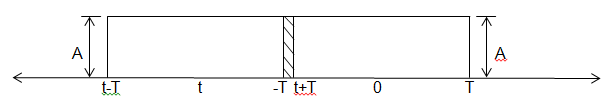
\includegraphics[scale=0.9]{fig3.png}
%\caption{\label VVoltage generator (side view)}
\end{figure}
This happens only for $t \in [-2T,2T]$\\
therefore for $t \in [-2T,0]$
\begin{eqnarray}
x_1(t)*x_2(t) &=& \int_{-\infty}^{\infty}x_1(\tau).x_2(t-\tau)d\tau\\
&=&\int_{-T}^{t+2T}A^2 d\tau \\
&=& A^2 (t+2T)
\end{eqnarray}
and for $t \in [0,2T]$
\begin{eqnarray}
x_1(t)*x_2(t) &=& \int_{-\infty}^{\infty}x_1(\tau).x_2(t-\tau)d\tau\\
&=&\int_{t-T}^{T}A^2 d\tau \\
&=& A^2 (2T-t)
\end{eqnarray}
\begin{figure}[ht]
\centering
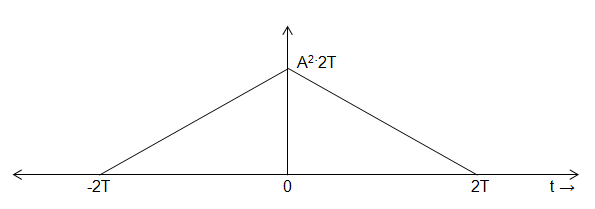
\includegraphics[scale=0.9]{fig4.png}
%\caption{\label VVoltage generator (side view)}
\end{figure}
\newpage
Now the Fourier transform of $x_1(t)*x_2(t)$ is
\[
= X_1(\Omega)X_2(\Omega)
\]
which is equal to
\[
\left( 2AT(\frac{\sin(\Omega T)}{\Omega T} \right) ^2
\] 

\subsection{The Principle of Duality}

We know that
\[
X(\Omega) = \int_{-\infty}^{\infty} \! x(t) e^{-j\Omega t} \ \mathrm{d}t
\]
and
\[
x(t) = \frac{1}{2\pi}\int_{-\infty}^{\infty} \! X(\Omega) e^{j\Omega t} \ \mathrm{d}\Omega
\]

Now, in the second integral, let's interchange $`t'$ and $`\Omega'$. Hence,
\[
x(\Omega) = \frac{1}{2\pi}\int_{-\infty}^{\infty} \! X(t) e^{j\Omega t} \ \mathrm{d}t
\]
Hence,
\[
x(-\Omega) = \frac{1}{2\pi}\int_{-\infty}^{\infty} \! X(t) e^{-j\Omega t} \ \mathrm{d}t
\]
Hence,
\[
2\pi [x(-\Omega)] = \int_{-\infty}^{\infty} \! X(t) e^{-j\Omega t} \ \mathrm{d}t
\]
This shows that, if
\[
x(t) \xrightarrow{\mathcal{F}} X(\Omega)
\]
then
\begin{equation}
X(t) \xrightarrow{\mathcal{F}} 2\pi [x(-\Omega)]
\end{equation}
This is the principle of duality for the Fourier transform. \\
\noindent
Let us take the example of the same rectangular pulse which we considered in the earlier section. The Fourier transform of the rectangular pulse is given by
\[
X(\Omega) = 2AT \frac{\sin(\Omega T)}{\Omega T}
\]
Let us invoke duality here. We will replace $T$ by $W$ for convenience of notation Hence,
\[
X(t) = 2AW \frac{\sin{(W t)}}{W t} \xrightarrow{\mathcal{F}} 2\pi [x(-\Omega)]
\]
Here, $2\pi x(\Omega)$ is the rectangular pulse with width $2W$ and height $2\pi A$. As the pulse is symmetric, $x(-\Omega) = x(\Omega)$.\\

We can see why this is a very useful property. Say you want to evaluate the convolution of $\sin(Wt)/Wt$. It is very difficult to evaluate it using the direct expression of the convolution. But, we can invoke the principle of duality here. We know that the Fourier transform of a convolution is the product of their Fourier transforms. Hence, applying this to $X(t)$,
\[
X(t)*X(t) \xrightarrow{\mathcal{F}} [2\pi x(\Omega)]^2
\]
Now, it is very easy to evaluate the right hand side. It is in fact the same symmetric rectangular pulse, but with height $(2\pi A)^2$. Hence, it is equal to $(2\pi)^2 A x(\Omega)$. Therefore, we have,
\begin{equation}
X(t)*X(t) \xrightarrow{\mathcal{F}} (2\pi)^2 A \ x(\Omega)
\end{equation}
Now, we know from the principle of duality (eq. (33)), that 
\[
X(t) \xrightarrow{\mathcal{F}} 2\pi [x(-\Omega)]
\]
Comparing this with eq. (34), we get,
\[
X(t)*X(t) = 2\pi A \ X(t) = 2\pi A \left( 2AW \frac{\sin(Wt)}{Wt} \right)
\]

Hence, the evaluation of the convolution of $\sin(Wt)/Wt$ and other complicated functions with themselves can become a lot easier and straightforward if we invoke the principle of duality.
